% Define the subtitle of the page
\title{Delving In}

% Begin the content of the page
\subsection{Delving In}

Edward's design reflects the building blocks for probabilistic
modeling. It defines interchangeable components, enabling rapid
experimentation and research with probabilistic models. Here we
provide an overview of the design.

Edward is named after the innovative statistician
\href{https://en.wikipedia.org/wiki/George_E._P._Box}{George Edward
Pelham Box}. Edward follows Box's philosophy of statistics and machine
learning.

First gather data from some real-world phenomena. Then cycle through
\href{http://www.annualreviews.org/eprint/7xbyci3nwAg5kEttvvjk/full/10.1146/annurev-statistics-022513-115657}
{Box's loop}:

\begin{enumerate}
\item Build a probabilistic model of the phenomena.
\item Reason about the phenomena given model and data.
\item Criticize the model, revise and repeat.
\end{enumerate}

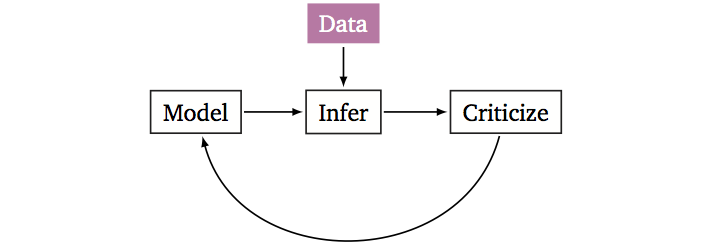
\includegraphics{images/model_infer_criticize.png}

Here's a toy example. A child flips a coin ten times, with the set of
outcomes being \texttt{{[}0,\ 1,\ 0,\ 0,\ 0,\ 0,\ 0,\ 0,\ 0,\ 1{]}},
where \texttt{0} denotes tails and \texttt{1} denotes heads. She
is interested in the probability that the coin lands heads. First,
build a model: assume the coin flips are independent and land heads with
the same probability. Second, reason about the phenomenon: use an algorithm
to infer the model given data. Third, criticize the model: analyze
whether the model captures the real-world phenomenon of coin flips. If it
doesn't, then revise the model and repeat.

This process defines the design of Edward. Four objects enable this
analysis.

\subsubsection{Data}

Data defines a set of observations. Edward represents
data as a Python dictionary, typically comprised of strings naming a
data object and NumPy arrays representing its values. For example,

\begin{lstlisting}[language=Python]
data = {'x': np.array([0, 1, 0, 0, 0, 0, 0, 0, 0, 1])}
\end{lstlisting}

Data can also store TensorFlow tensors to contend with situations where the
observations do not fit in memory.

\subsubsection{Models}\label{models}

A probabilistic model is a joint distribution $p(x, z)$ of data $x$ and latent
variables $z$.
Edward supports several languages for specifying probability models:
TensorFlow, Python, PyMC3, and Stan. In general, a probability
model is a class with structure
\begin{lstlisting}[language=Python]
class Model:
    def __init__(...):
        ...
        self.n_vars = ...

    def log_prob(self, xs, zs):
        log_prior = ...
        log_likelihood = ...
        return log_prior + log_likelihood

model = Model(...)
\end{lstlisting}
The field \texttt{n\_vars} denotes the number of latent variables in the
probability model. For example, a model with a Gaussian likelihood with latent
mean and variance would have \texttt{n\_vars=2*N} latent variables for
\texttt{N} observations.

The method \texttt{log_prob(xs, zs)} calculates the log probability of
the joint density $\log p(x,z)$. Here \texttt{xs} can be a single data
point or a batch of data points. Analogously, \texttt{zs} can be a
single set of latent variables, or a batch thereof. The method returns a vector
of log density evaluations, one for each set of latent variables.

\subsubsection{Inference}\label{inference}

Given a model and data, we aim to
reason about $z$: the model's hidden structure. The
posterior distribution $p(z \mid x)$ captures our reasoning: its mean
describes our best guess of the hidden structure, and its variance
describes the uncertainty around our best guess.

%The posterior distribution is typically intractable.
Edward has many inference algorithms and makes it easy
to develop new ones.

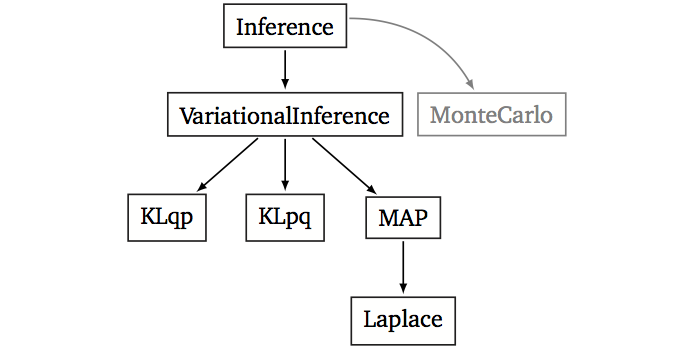
\includegraphics{images/inference_structure.png}
{\small\textit{Dependency graph of inference methods.
Nodes are classes in Edward and arrows represent class inheritance.}}

Edward focuses on variational inference. It views posterior inference
as positing a model of the latent variables $q(z \;;\; \lambda)$ and optimizing it to
approximate the posterior $p(z \mid x)$.
%which seeks to match the variational model  to the
%posterior of the probability model.


Edward provides a library of
\texttt{RandomVariable} objects. Variational models use these to infer
each latent variable in the probability model.
For example, to specify a variational model (e.g.~for a Gaussian mixture)
\begin{align*}
  q(z \;;\; \lambda)
  &=
  \text{Dirichlet}(z_\pi)
  \times
  \mathcal{N}(z_\mu)
  \times
  \text{InvGamma}(z_\sigma)
\end{align*}
we would write
\begin{lstlisting}[language=Python]
from edward.models import Dirichlet, Normal, InvGamma

qpi = Dirichlet(K)
qmu = Normal(K*D)
qsigma = InvGamma(K*D)
\end{lstlisting}

Each algorithm derived from \texttt{VariationalInference} minimizes a
different loss function between the variational model and the
posterior.
%They take as input a probability model \texttt{model}, a
%variational model \texttt{variational}, and data \texttt{data}.
For example, to minimize the Kullback-Leibler divergence
\begin{align*}
  \text{KL}(p(z \mid x) \;\|\; q(z \;;\; \lambda))
\end{align*}
we first instantiate the inference class: bind each latent variable to
its corresponding variational distribution; then pass in data and the
model; then run it.
\begin{lstlisting}[language=Python]
inference = ed.KLpq({'pi': qpi, 'mu': qmu, 'sigma': qsigma}, data, model)
inference.run(n_iter=500, n_minibatch=5)
\end{lstlisting}
This runs the \texttt{KLpq} minimization algorithm for \texttt{500} iterations,
using a batch of \texttt{5} data points per iteration.

\subsubsection{Criticism}\label{criticism}

Criticizing models and their inference is a crucial step in analysis.
Following falsificationists such as Popper and Box, no model will exactly
describe the natural phenomena we seek to analyze; in other words, ``all models
are wrong''. Thus we would like to uncover where and how the model goes wrong.

Edward explores model and inference criticism using
\begin{itemize}
  \item point-based evaluations, such as mean squared error or
  classification accuracy
\end{itemize}
\begin{lstlisting}[language=Python]
ed.evaluate('mean_squared_error', data={'y': y_train, 'x': x_train},
            latent_vars={'z': qz}, model_wrapper=model)
\end{lstlisting}
\begin{itemize}
  \item posterior predictive checks, for making probabilistic
  assessments of the model fit using discrepancy functions
\end{itemize}
\begin{lstlisting}[language=Python]
T = lambda xs, zs: tf.reduce_mean(xs['x'])
ed.ppc(T, data={'x': x_train}, latent_vars={'z': qz}, model_wrapper=model)
\end{lstlisting}

See the \href{tutorials}{tutorials} for examples of models,
inference, and criticism in Edward.

See the \href{api/}{API} for details of how Edward implements these
objects.

\subsubsection{References}\label{references}

\begin{itemize}
\item
  Box, G.E.P. (1976). Science and Statistics. Journal of the American
  Statistical Association, 71(356), 791–799
\item
  David M Blei. (2014). Build, compute, critique, repeat: Data analysis with
  latent variable models. Annual Review of Statistics, 1:203-232
\end{itemize}
